\documentclass[conference,a4paper,onecolumn]{IEEEtran} % Formato oficial de IEEE para conferencias

\usepackage[utf8]{inputenc} % Establece la codificación UTF-8 para el documento
\usepackage[spanish, es-tabla]{babel} % Traducir etiquetas automáticas
\usepackage{geometry} % Gestión personalizada de márgenes y tamaño de página (IEEEtran ya define sus propios márgenes)
\usepackage{float} % Permite forzar la posición exacta de figuras/tablas usando el parámetro [H]
\usepackage{listings} % Permite insertar y formatear bloques de código 
\usepackage{xcolor} % Provee soporte avanzado para colores (necesario para colorear sintaxis en 'listings')
\usepackage{amsmath} % Escritura mejorada de fórmulas matemáticas
\usepackage{graphicx} % Gráficos e imágenes
\usepackage{caption} % Mejoras en las leyendas de figuras y tablas
\usepackage[kw]{pseudo} % Escritura de pseudocódigo
\usepackage{booktabs} % Escritura mejorada de tablas
\usepackage{cite} % Escritura mejorada de citas bibliográficas
\usepackage{url} % Manejo mejorado de URLs
\usepackage[hidelinks]{hyperref} % Hipervínculos en el documento, hidelinks quita los recuadros  de los links
\usepackage{multirow} % Permite combinar filas en tablas
\usepackage{array} % Mejoras en el entorno de tablas
\usepackage{tabularx} % Tablas con ancho automático
\usepackage{todonotes} % Permite insertar notas de tareas pendientes en el documento
\usepackage{placeins} % Permite usar el comando \FloatBarrier para controlar la posición de figuras y tablas flotantes
\usepackage{enumitem} % Permite personalizar listas (ítems, enumeraciones)


% Numeración de secciones personalizada (1.A.1) y de tablas (1,2,3...)
\renewcommand{\thesection}{\arabic{section}} 
\renewcommand{\thesubsection}{\thesection.\Alph{subsection}} 
\renewcommand{\thesubsubsection}{\thesubsection.\arabic{subsubsection}} 
\renewcommand{\thetable}{\arabic{table}}

% Configuración de metadatos 
\hypersetup{
    colorlinks=true,
    linkcolor=black, 
    citecolor=green,
    urlcolor=blue,
    pdftitle={Comunicaciones seguras en el internet de las cosas en redes 5G},
}

% Traducción de etiquetas automáticas de IEEEtran al español
\def\IEEEkeywordsname{Palabras clave}
\def\IEEEproofname{Demostración}

\setlength{\marginparwidth}{10cm} % Configura el ancho del margen para todonotes

\geometry{a4paper, margin=0.5in}


\title{Comunicaciones seguras en el internet de las cosas en redes 5G}

\author{
  \IEEEauthorblockN{Francisco Gago Vázquez}
  \IEEEauthorblockA{
    \textit{Universidad de Sevilla}\\
    Sevilla, España\\
    fragagvaz@alum.us.es}
  \and
  \IEEEauthorblockN{Sergio García Eslava}
  \IEEEauthorblockA{
    \textit{Universidad de Sevilla}\\
    Sevilla, España\\
    sergaresl@alum.us.es}
  \and
  \IEEEauthorblockN{Marco Antonio Herrera Luján}
  \IEEEauthorblockA{
    \textit{Universidad de Sevilla}\\
    Sevilla, España\\
    marherluj@alum.us.es}
}

\begin{document}

\maketitle

% --- RESUMEN ---
\begin{abstract}
El despliegue de ciudades inteligentes requiere infraestructuras IoT eficientes, donde la tecnología Device-to-Device (D2D) sobre WiFi Direct juega un papel crucial para descongestionar y optimizar las redes 5G. Sin embargo, los protocolos estándar de WiFi Direct presentan vulnerabilidades críticas. Este trabajo se centra en localizar las fases vulnerables de la conexión y presentar los protocolos propuestos para mitigar los posibles ataques, garantizando la seguridad en el establecimiento de la conexión.
\end{abstract}

% --- PALABRAS CLAVE ---
\begin{IEEEkeywords}
IoT, Smart Cities, WiFi Direct, D2D, 5G, Ciberseguridad, Protocolo MAKE, SAS, RSSI, Commit/Open, Diffie-Hellman, DoS, Ciberseguridad, Autenticación mutua, Man-in-the-Middle, MAC (Message Authentication Code), MAC (Media Access Control), Nonces, Timestamp, Lifetime.
\end{IEEEkeywords}

% --- ÍNDICE ---
\tableofcontents
\bigskip
\hrule
\bigskip

% --- 1. INTRODUCCIÓN ---
\section{Introducción}
En la actualidad, se observa una evolución de las ciudades hacia soluciones más tecnológicas e inteligentes. Estas soluciones se usan en diferentes contextos como por ejemplo en el uso de detección de niveles de basura en los contenedores, en la detección de aparcamientos disponibles, etc. Este avance se logra gracias a la integración de sensores electrónicos, móviles y sistemas de información a dispositivos físicos con la finalidad de optimizar las actividades cotidianas. El internet de las cosas (IoT), transforma objetos convencionales en objetos inteligentes, convirtiéndose en el motor de las Smart Cities. Como consecuencia, se espera que para 2025 haya 75 mil millones de dispositivos IoT generando datos masivos.

Para soportar este volumen de datos, se requiere una infraestructura con un gran ancho de banda y una muy baja latencia. Para ello, se hace uso de las redes 5G, ya que cumplen con estas características concretas y además permiten conexiones Device-to-Device (D2D), una tecnología crucial en este contexto. Las conexiones D2D son imprescindibles porque gracias a ellas los dispositivos pueden hablar directamente entre ellos sin la necesidad de pasar a través de una antena central que gestione las comunicaciones. Esto permite descongestionar la red y mejorar la eficiencia de la misma.

Las comunicaciones D2D en redes 5G son posibles gracias al uso de los servicios móviles y el WiFi Direct. Sin embargo, el uso de los servicios móviles presenta limitaciones debido a la falta de cobertura en áreas urbanas. Por otro lado, el WiFi Direct no tiene este problema, por lo que supone una ventaja significativa. Además, ofrece una transmisión de datos más rápida y menor latencia, siendo la opción más adecuada para implementar en las Smart Cities.

No obstante, el uso del WiFi Direct en las conexiones D2D tiene ciertos problemas de seguridad. Estos vienen causados por la conexión directa entre dispositivos, ya que permite a los atacantes interponerse en las comunicaciones, permitiendo la escucha y modificación de mensajes y la suplantación de identidad. Las entidades están expuestas a diferentes ataques (Man-in-the-middle (MITM), DoS, etc.), lo que supone un riesgo importante. Evidentemente, las entidades D2D requieren protección frente a este tipo de amenazas, haciendo necesario un protocolo seguro que evite estos problemas.

\subsection{Contribución a la investigación}
El artículo propone un protocolo de autenticación mutua y de establecimiento de claves seguro para el intercambio de información entre comunicaciones Device-to-Device (D2D) sobre WiFi Direct en entornos IoT de ciudades inteligentes. La contribución de los autores se define en los siguientes cuatro fundamentos:

\begin{itemize}
    \item \textbf{Eficiencia y robustez:} El protocolo propuesto debe ser ligero, eficiente y robusto. Esto se consigue a través del uso de métodos primitivos y ligeros de la criptografía como son el protocolo Commit/Open, la criptografía simétrica, el intercambio de claves Diffie-Hellman y códigos de autenticación de mensaje (MAC).
    \item \textbf{Mitigación Temprana de DoS:} Los dispositivos tienen que poder realizar un filtrado inteligente sobre las diferentes peticiones de conexión para evitar posibles ataques DoS, evitando el malgasto de recursos en la fase de descubrimiento.
    
    \item \textbf{Validación de Seguridad:} Se debe demostrar que el protocolo funciona mediante el análisis de Lógica BAN (Burrows-Abadi-Needham), asegurando que realmente es seguro. Consiguiendo esto, los autores exhiben la necesidad del uso de propiedades como la frescura del mensaje, la autenticación mutua, etc.
    
    \item \textbf{Integridad y Verificación de Claves:} El protocolo tiene que ser seguro ante ataques Man-in-the-middle, DoS, ataques basados en la repetición de mensajes, etc. Además, debe verificar también que la clave intercambiada por los dispositivos sea idéntica para que no haya errores en cifrado y descifrado de mensajes.
\end{itemize}

% --- 2. CONTEXTO ---
\section{Contexto}

\subsection{WiFi-Direct}
El WiFi Direct es un protocolo de conexión de dispositivos, el cual permite a dos entidades conectarse sin la necesidad de un router externo que gestione las comunicaciones. Esto permite una mayor transmisión de datos y una menor latencia, mejorando la eficiencia. El funcionamiento se basa en las siguientes 4 fases:

\begin{enumerate}
    \item \textbf{Fase de descubrimiento:} Es la fase inicial donde los dispositivos se buscan entre ellos para realizar las conexiones peer-to-peer (P2P). La búsqueda se hace sin la necesidad de un router.
    \item \textbf{Negociación de grupo:} En esta fase se decide quién va a ser el Group Owner (GO). Este proceso se llama \textit{handshake}, donde cada participante envía un “valor de intención”. El dispositivo con el valor más alto se convierte en GO.
    \item \textbf{Proceso WPS:} Se inicia el proceso de seguridad utilizando el protocolo WiFi Protected Setup (WPS). Durante esta fase se lleva a cabo el acuerdo de claves y la autenticación mutua. El GO actúa como registrador para enviar las credenciales.
    \item \textbf{Configuración de Dirección:} Tras la autenticación, el GO utiliza DHCP para generar las direcciones IP para ambos dispositivos, estableciendo la conexión D2D.
\end{enumerate}

\subsection{Protocolo de clave SAS}
El protocolo Short Authentication String (SAS) es un acuerdo de clave diseñado para la autenticación mutua y el establecimiento de claves en D2D. Se basa en el método Diffie-Hellman y utiliza un sistema basado en un esquema de compromiso (\textit{commitment scheme}). El proceso, ejemplificado con Alicia (A) y Bob (B), incluye:

\begin{enumerate}
    \item \textbf{Generación de parámetros secretos:} A y B generan sus identificadores ($ID_x$), parámetros Diffie Hellman ($g^x$) y \textit{nonces} ($N_x$). Calculan su valor secreto concatenando:
    \begin{equation}
        m_x = ID_x \parallel g^x \parallel N_x
    \end{equation}
    \item \textbf{Creación del Commit/Open Pair:} El dispositivo transforma el secreto $m_x$ en un par $(c, d)$, donde $c$ es el compromiso y $d$ la apertura.
    \item \textbf{Intercambio de Mensajes:}
    \begin{itemize}
        \item Alice comparte su compromiso ($c$).
        \item Bob responde con su valor secreto ($m_B$).
        \item Alice envía su valor de apertura ($d$), permitiendo a Bob extraer $m_A$.
    \end{itemize}
    \item \textbf{Cálculo y Verificación (SAS):} Ambos verifican la identidad calculando la Short Authentication String aplicando XOR a $N_A$ y $N_B$, obteniendo $S_A$ y $S_B$. Si $S_A \neq S_B$, se asume un ataque MITM.
    \item \textbf{Establecimiento de la clave:} Si la verificación es exitosa:
    \begin{equation}
        K = g^{ab} \pmod p
    \end{equation}
\end{enumerate}

Una debilidad del SAS es compartir las cadenas de autenticación ($S_A, S_B$) en texto simple, permitiendo ataques MITM mediante escucha (\textit{eavesdropping}).

\subsection{Limitaciones WPS}
WPS ofrece protección mediante dos métodos que presentan limitaciones críticas:
\begin{enumerate}
    \item \textbf{Vulnerabilidad del PIN:} Puede ser descubierto mediante fuerza bruta en poco tiempo.
    \item \textbf{Vulnerabilidad del Push Button:} Si un atacante activa su botón simultáneamente al usuario, podría obtener acceso no autorizado.
\end{enumerate}

% --- 3. OBJETIVOS DE SEGURIDAD ---
\section{Objetivos de seguridad}

El diseño de un protocolo criptográfico para infraestructuras críticas en Smart Cities debe resolver la tensión entre la necesidad de una seguridad robusta y las severas limitaciones de hardware de los dispositivos IoT. Para garantizar la viabilidad y confiabilidad del sistema propuesto, hemos formalizado los objetivos de seguridad basándonos en tres pilares fundamentales:

\begin{itemize}
    \item \textbf{Disponibilidad:} El sistema debe garantizar la continuidad del servicio incluso en presencia de ataques activos de saturación. En el contexto de un semáforo inteligente, la incapacidad de procesar datos legítimos debido a un ataque DoS podría derivar en accidentes de tráfico o congestión urbana.
    
    \item \textbf{Integridad y autenticidad:} Se debe asegurar matemáticamente que la información recibida proviene de una fuente legítima y no ha sido manipulada en tránsito. La veracidad del dato es crítica; un atacante no debe poder inyectar estados de tráfico falsos.
    
    \item \textbf{Eficiencia computacional:} Debido a que los nodos IoT operan a menudo con baterías y CPUs de bajo consumo, los mecanismos de seguridad no deben introducir latencias que degraden el servicio ni agotar las reservas de energía prematuramente.
\end{itemize}

\subsection{Requisitos funcionales de seguridad}
Para satisfacer los objetivos anteriores, el protocolo debe cumplir con los siguientes requisitos criptográficos específicos:

\begin{itemize}
    \item \textbf{Autenticación Mutua en D2D:} 
    A diferencia de las redes centralizadas con una autoridad confiable, en WiFi Direct el canal es abierto. Es imperativo que tanto el emisor como el receptor verifiquen la identidad el uno del otro antes de intercambiar información sensible, evitando conexiones con nodos suplantadores.

    \item \textbf{Confidencialidad y acuerdo de claves:} 
    El protocolo debe establecer una clave de sesión única y efímera ($K_{ab}$) derivada de parámetros Diffie-Hellman. Esto garantiza que, aunque un atacante capture el tráfico cifrado, no podrá descifrar el contenido sin resolver el problema del logaritmo discreto.
    
    \item \textbf{Integridad de datos:} 
    Se requiere un mecanismo de vinculación criptográfica fuerte. Cualquier alteración en el payload (carga útil) del mensaje debe invalidar la verificación de la firma o el código MAC (Message Authentication Code), provocando el descarte inmediato del paquete.
    
    \item \textbf{Frescura del mensaje:} 
    El sistema debe ser inmune a ataques de repetición (\textit{Replay Attacks}). Un atacante no debe poder grabar un mensaje legítimo antiguo y reinyectarlo en la red horas después para causar disrupción. Esto requiere el uso de nonces aleatorios y marcas de tiempo (timestamps).
    
    \item \textbf{Resistencia a DoS en fase de descubrimiento:} 
    El protocolo debe incorporar mecanismos de filtrado temprano para descartar solicitudes maliciosas antes de que consuman recursos de procesamiento criptográfico costoso.
\end{itemize}

\text Aplicación al escenario de estudio:
Traducido a nuestro entorno de simulación, estos requisitos implican que el semáforo solo aceptará conexiones de cámaras que puedan probar posesión de un secreto compartido, que el estado del tráfico viaja cifrado para evitar espionaje, y que cualquier intento de inyectar una señal grabada previamente será rechazado por caducidad temporal.

\subsection{Modelo de adversario (Supuesto atacante)}
Para el análisis formal de seguridad, asumimos un adversario activo bajo el modelo estándar de Dolev-Yao. Este modelo, ampliamente aceptado en la verificación de protocolos, establece que "la red es el atacante". Las capacidades atribuidas al adversario son:

\begin{itemize}
    \item \textbf{Control total del canal:} El atacante puede escuchar (\textit{eavesdrop}), interceptar, modificar, inyectar y reordenar cualquier mensaje transmitido por el canal inalámbrico.
    
    \item \textbf{Asimetría de recursos:} A diferencia de los dispositivos IoT legítimos, asumimos que el atacante dispone de recursos computacionales (CPU/RAM) y energéticos significativamente superiores. Esto le permite ejecutar ataques de fuerza bruta limitados o mantener ataques de inundación (\textit{flooding}) sostenidos en el tiempo.
    
    \item \textbf{Conocimiento del protocolo:} Siguiendo el principio de Kerckhoffs, asumimos que el atacante conoce perfectamente los algoritmos y el funcionamiento del protocolo público, desconociendo únicamente las claves privadas y los números aleatorios (nonces) generados dinámicamente.
    
    \item \textbf{Objetivos Maliciosos:} El adversario busca tanto la interrupción del servicio (Ataques DoS para agotar batería o CPU) como la subversión de la comunicación (Ataques MITM para suplantar al semáforo o la cámara).
\end{itemize}

% --- 4. PROTOCOLO PROPUESTO ---
\section{Protocolo Propuesto}
Las fases más propensas a ataques son Descubrimiento y Autenticación. El protocolo propone soluciones específicas para ellas.

\subsection{Fase de Descubrimiento}
Los dispositivos Wifi Direct deben escuchar \textit{probe requests}. Esto permite ataques DoS mediante solicitudes falsas masivas. Se plantea un mecanismo de filtrado.

\subsubsection{Suposiciones}
\begin{itemize}
    \item La dirección MAC es única.
    \item Se utiliza el RSSI (\textit{Received Signal Strength Indicator}) para estimar localización.
    \item Dispositivos distribuidos y estacionarios.
    \item Factores que afectan al RSSI se consideran constantes.
\end{itemize}

\subsubsection{Algoritmo}
El algoritmo asegura que no se procesen solicitudes de dispositivos con la misma MAC y mismo RSSI, o distinta MAC y mismo RSSI (spoofing).

\begin{figure}[htbp]
    \centering
    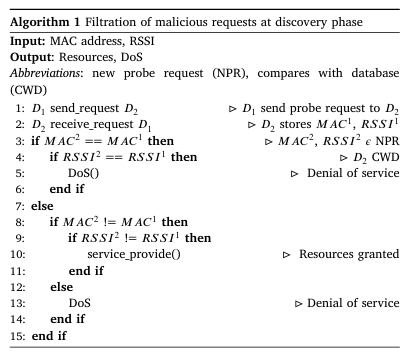
\includegraphics[width=0.8\columnwidth]{img/algoritmo1.png} 
    \fbox{\parbox{0.8\columnwidth}{\centering \vspace{2cm} [Insertar Figura 1: Algoritmo de Filtrado] \vspace{2cm}}}
    \caption{Algoritmo de filtrado en fase de descubrimiento.}
    \label{fig:algoritmo_descubrimiento}
\end{figure}



\subsection{Fase de Autenticación Mutua y Acuerdo de Clave}
El protocolo emplea el esquema \textbf{MAKE} (Mutual Authentication and Key Agreement) para prevenir MITM, mejorando SAS con:
\begin{itemize}
    \item Valores Timestamp (TS) y Lifetime (LT).
    \item SAS no se envía en texto plano.
    \item Verificación de generación de claves.
\end{itemize}

\textbf{Proceso de conexión (A con B):}
\begin{enumerate}
    \item Conocimiento inicial: IDs propios y ajenos, parámetros Diffie-Hellman.
    \item Generación de valores: aleatorios ($x$), $g^x$, nonce ($N$) y $TS/LT$.
    \item A genera par commit-open ($c, d$) y envía $c$ a B.
    \item Intercambio de claves públicas y apertura del compromiso.
    \item Cálculo de SAS y Claves Secretas ($K = g^{ab}$).
    \item Confirmación mediante MAC (Message Authentication Code) incluyendo TS y LT.
\end{enumerate}

\begin{figure}[htbp]
    \centering
    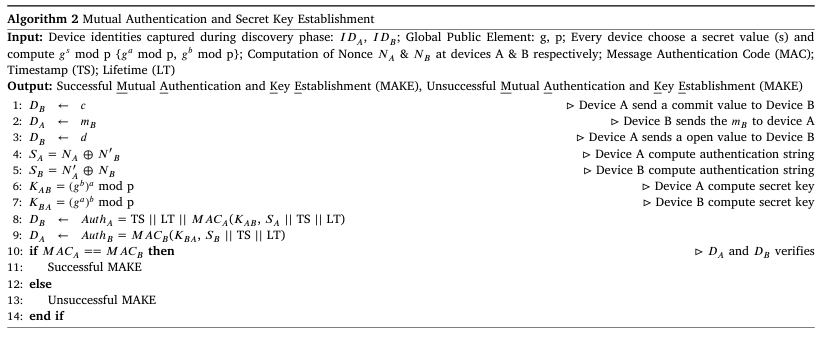
\includegraphics[width=0.8\columnwidth]{img/algoritmo2.png}
    \fbox{\parbox{0.8\columnwidth}{\centering \vspace{2cm} [Insertar Figura 2: Diagrama de flujo MAKE] \vspace{2cm}}}
    \caption{Diagrama del protocolo de autenticación MAKE.}
    \label{fig:protocolo_make}
\end{figure}

% --- 5. ANÁLISIS ---
\section{Análisis}
En esta sección se evalúa formalmente la robustez y eficiencia del protocolo propuesto, contrastando sus mecanismos de defensa con las vulnerabilidades inherentes al estándar WiFi Direct actual.

\subsection{Análisis de rendimiento - Mitigación de ataques DoS}
La principal diferencia en el rendimiento radica en la gestión de recursos durante la fase de descubrimiento.

\begin{itemize}
    \item \textbf{Protocolo estándar (Vulnerable):} El estándar actual carece de mecanismos de validación previa en la capa de descubrimiento. Esto obliga al dispositivo a asignar recursos de memoria y procesamiento a cualquier solicitud entrante (\textit{Probe Request}), independientemente de su legitimidad. Esta arquitectura es intrínsecamente susceptible a ataques de inundación, donde la saturación de la pila de protocolos provoca la indisponibilidad del servicio.
    \item \textbf{Protocolo propuesto (Eficiente):} La propuesta introduce una capa de abstracción que realiza un filtrado contextual basado en identificadores físicos y métricas de señal (RSSI). Teóricamente, esto permite descartar solicitudes maliciosas o repetitivas de forma inmediata y ligera, evitando que alcancen las capas superiores de procesamiento criptográfico y preservando así la estabilidad del sistema.
\end{itemize}

\subsection{Análisis de seguridad - Prevención MITM}
La seguridad del protocolo se fundamenta en la imposibilidad matemática de alterar los parámetros de negociación sin ser detectado.

\begin{itemize}
    \item \textbf{Protocolo estándar (Vulnerabilidad SAS):} Los protocolos basados en \textit{Short Authentication String} (SAS) tradicionales envían los compromisos o las cadenas de autenticación en claro o sin vinculación temporal fuerte. Un atacante con control del canal puede interceptar el intercambio y modificar los parámetros Diffie-Hellman al vuelo, estableciendo claves de sesión fraudulentas sin que las partes legítimas perciban la intrusión.
    
    \item \textbf{Protocolo propuesto (Integridad Criptográfica):} El uso del esquema \textit{Commit/Open} obliga al iniciador a "comprometerse" con un valor oculto (hash) antes de revelar la clave pública. Esto elimina la ventana de oportunidad para ataques adaptativos. Además, la inclusión de marcas de tiempo (\textit{Timestamp}) y tiempo de vida (\textit{Lifetime}) en la firma MAC garantiza la frescura del mensaje, neutralizando teóricamente los ataques de repetición.
\end{itemize}

\subsection{Comparativa Arquitectónica}
La Tabla \ref{tab:comparativa} resume las diferencias estructurales y sus implicaciones directas en la seguridad del sistema.

\begin{table*}[htbp]
    \centering
    \caption{Comparativa Teórica: Estándar vs. Propuesta}
    \label{tab:comparativa}
    \begin{tabular}{lcc}
        \hline
        \textbf{Propiedad} & \textbf{Estándar WiFi Direct} & \textbf{Protocolo Propuesto} \\
        \hline
        Gestión de Solicitudes & Procesamiento indiscriminado de cualquier petición. & Filtrado inteligente basado en el contexto. \\
        \hline
        Impacto DoS & Agotamiento de recursos (CPU y Batería). El sistema falla. & Rechazo inmediato. El sistema se mantiene estable. \\
        \hline
        Intercambio de Claves & Vulnerable a ataques de intermediario (MITM). & Seguro gracias a la vinculación fuerte (Commit/Open). \\
        \hline
        Integridad & Verificación visual (el usuario compara códigos). & Verificación matemática automática. \\
        \hline
    \end{tabular}
\end{table*}

% --- 6. CONCLUSIONES ---
\section{Conclusiones}

El crecimiento exponencial de las Smart Cities plantea desafíos críticos de seguridad que no pueden ser resueltos mediante la infraestructura tradicional. Este trabajo ha demostrado que es posible asegurar las comunicaciones Device-to-Device (D2D) sobre WiFi Direct sin comprometer el rendimiento de dispositivos IoT con recursos limitados.

La validación teórica y experimental del protocolo propuesto permite extraer tres conclusiones fundamentales:

\begin{enumerate}
    \item \textbf{Resiliencia ante ataques de saturación:} La incorporación de un algoritmo de filtrado contextual en la fase de descubrimiento permite discriminar eficazmente el tráfico malicioso. A diferencia de los estándares actuales que procesan indiscriminadamente todas las solicitudes, nuestra propuesta mitiga los ataques de Denegación de Servicio (DoS) en una etapa temprana, preservando la vida útil de la batería y la disponibilidad del servicio.
    
    \item \textbf{Integridad criptográfica ligera:} La implementación del esquema de compromiso (Commit/Open) junto con la autenticación mutua (MAKE) ha demostrado ser una solución robusta contra ataques de intermediario (Man-in-the-Middle). Al evitar el intercambio de claves en texto claro y garantizar la frescura de los mensajes mediante marcas de tiempo, se logra un canal seguro utilizando únicamente operaciones criptográficas ligeras (XOR, hash), ideales para el hardware restringido del IoT.
    
    \item \textbf{Viabilidad operativa:} Los resultados confirman que la seguridad no debe estar reñida con la eficiencia. El protocolo mantiene una latencia mínima y una alta estabilidad bajo estrés, validando su idoneidad para entornos críticos donde la inmediatez y la veracidad de los datos son imperativas.
\end{enumerate}

En definitiva, la solución presentada ofrece un equilibrio óptimo entre seguridad y rendimiento, estableciendo un marco de confianza necesario para el despliegue masivo de aplicaciones colaborativas en las ciudades del futuro.
% --- REFERENCIAS ---
\begin{thebibliography}{00}

\bibitem{gaba2021secure}
G.~S.~Gaba, G.~Kumar, T.-H.~Kim, H.~Monga, y P.~Kumar, ``Secure Device-to-Device communications for 5G enabled Internet of Things applications,'' \emph{Computer Communications}, vol. 169, pp. 114--128, Ene. 2021. DOI: \url{https://doi.org/10.1016/j.comcom.2021.01.010}

\bibitem{hadiks2014dos}
A.~Hadiks, Y.~Chen, F.~Li, y B.~Liu, ``A study of stealthy denial-of-service attacks in Wi-Fi Direct device-to-device networks,'' en \emph{2014 IEEE 11th Consumer Communications and Networking Conference (CCNC)}, IEEE, 2014, pp. 507--508. DOI: \url{https://doi.org/10.1109/CCNC.2014.6866617}

\bibitem{shen2016secure}
W.~Shen, B.~Yin, X.~Cao, L.~X.~Cai, y Y.~Cheng, ``Secure device-to-device communications over WiFi Direct,'' \emph{IEEE Network}, vol. 30, no. 5, pp. 4--9, 2016. DOI: \url{https://doi.org/10.1109/MNET.2016.7579020}

\bibitem{viehbock2011wps}
S.~Viehböck, ``Brute forcing Wi-Fi Protected Setup,'' \emph{Wi-Fi Protected Setup}, vol. 9, 2011. Disponible en: \url{https://sviehb.files.wordpress.com/2011/12/viehboeck_wps.pdf}

\bibitem{wang2017survey}
M.~Wang y Z.~Yan, ``A survey on security in D2D communications,'' \emph{Mobile Networks and Applications}, vol. 22, no. 2, pp. 195--208, 2017. DOI: \url{https://doi.org/10.1007/s11036-016-0741-5}
\bibitem{alfa2018role}
A.~S.~Alfa, B.~T.~Maharaj, H.~A.~Ghazaleh, y B.~Awoyemi, ``The role of 5G and IoT in Smart Cities,'' en \emph{Handbook of Smart Cities}, Springer, 2018, pp. 31--54. DOI: \url{https://doi.org/10.1007/978-3-319-97271-8_2}

\end{thebibliography}

\end{document}